\documentclass[
  a4paper,
  12pt,
  english,
  brazilian,
]{article}

%% Pacotes utilizados
\usepackage[]{fatec-article}
\usepackage{float} % ← ADICIONE ESTE PACOTE

%% Início do documento
\begin{document}
\vspace{8cm}
\begin{center}
    \large \textbf{\title{ARTEFATOS DO PROJETO DE SOFTWARE}}
\end{center}

\maketitle
\break
\tableofcontents
\break

\section*{Diagramas UML}
    Diagramas UML (Unified Modeling Language) são ferramentas visuais para modelar a estrutura e o comportamento de sistemas de software. No nosso caso foi desenvolvido o diagrama de Objeto.
    
    \subsection*{Diagrama de Objetos}
    \addcontentsline{toc}{section}{Diagrama de Objetos}

    Um diagrama de objetos é uma representação visual de um sistema em um momento específico, mostrando instâncias concretas de objetos e os relacionamentos entre elas.

\begin{figure}[H] % ← TROQUE [h] por [H]
\centering
\caption{Diagrama de objetos}
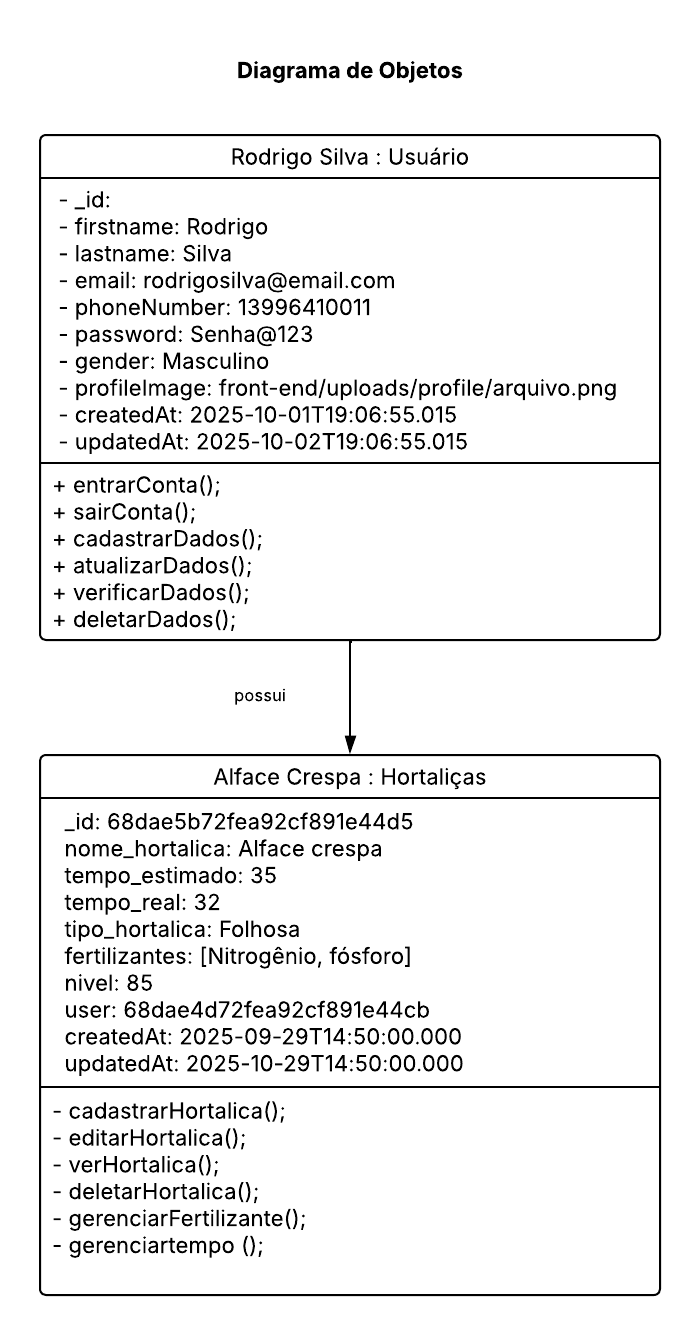
\includegraphics[scale=0.5]{Logos/PI - Diagrama de Objetos.png}
\SourceOrNote{Autoria própria (2025)}
\end{figure}

    No contexto da Fazenda Vertical orientada por Redes Neurais foram mapeadas as principais necessidades do usuário. Desta forma, identificamos a necessidade de duas coleções de dados (para usuário e vegetais), 6 ações do usuário (login, logout, cadastro, atualização, verificação e deleção de dados) e 6 para os vegetais (cadastro, edição, verificação, deleção, gerenciamento do tempo e gerencimento de fertilizante).
    
\section*{Diagrama de banco de dados}
\addcontentsline{toc}{section}{Diagrama de banco de dados}
Um diagrama de banco de dados é um esquema visual que representa a estrutura lógica de um banco de dados, mostrando as tabelas, suas colunas, atributos e como elas se relacionam entre si.

\begin{figure}[H] % ← TROQUE [!ht] por [H]
\centering
\caption{Diagrama de Banco de Dados}
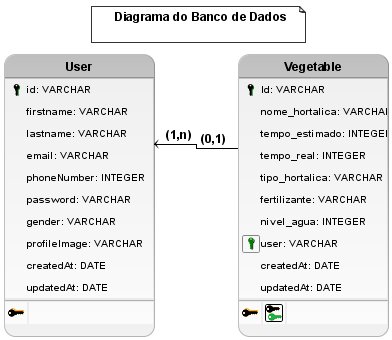
\includegraphics[scale=0.6]{Logos/PI - Diagrama de Banco de Dados.png}
\SourceOrNote{Autoria própria (2025)}
\end{figure}

Em nosso projeto foi utilizado um banco de dados não-relacional e foram mapeadas 2 coleções (user e vegetable). Na coleção user temos as chaves: \texttt{\_id: ObjectId}, \texttt{firstname: String} (Nome do usuário - obrigatório), \texttt{lastname: String} (Sobrenome do usuário - obrigatório), \texttt{email: String} (E-mail único - obrigatório, lowercase), \texttt{phoneNumber: String} (Telefone - obrigatório), \texttt{password: String} (Senha - mínimo 6 caracteres), \texttt{gender: String} (Gênero: ['masculino', 'feminino', 'outro']), \texttt{profileImage: String} (Caminho da imagem de perfil), \texttt{createdAt: Date} (Data de criação - automático), \texttt{updatedAt: Date} (Data de atualização - automático).

\section*{CANVAS}
\addcontentsline{toc}{section}{CANVAS}
Canvas é um mapa visual para descrever e analisar um modelo de negócios, composto por nove blocos interligados que cobrem aspectos como segmentos de clientes, proposta de valor, canais, fontes de receita e recursos.

\begin{figure}[H] % ← TROQUE [!ht] por [H]
\centering
\caption{CANVAS}
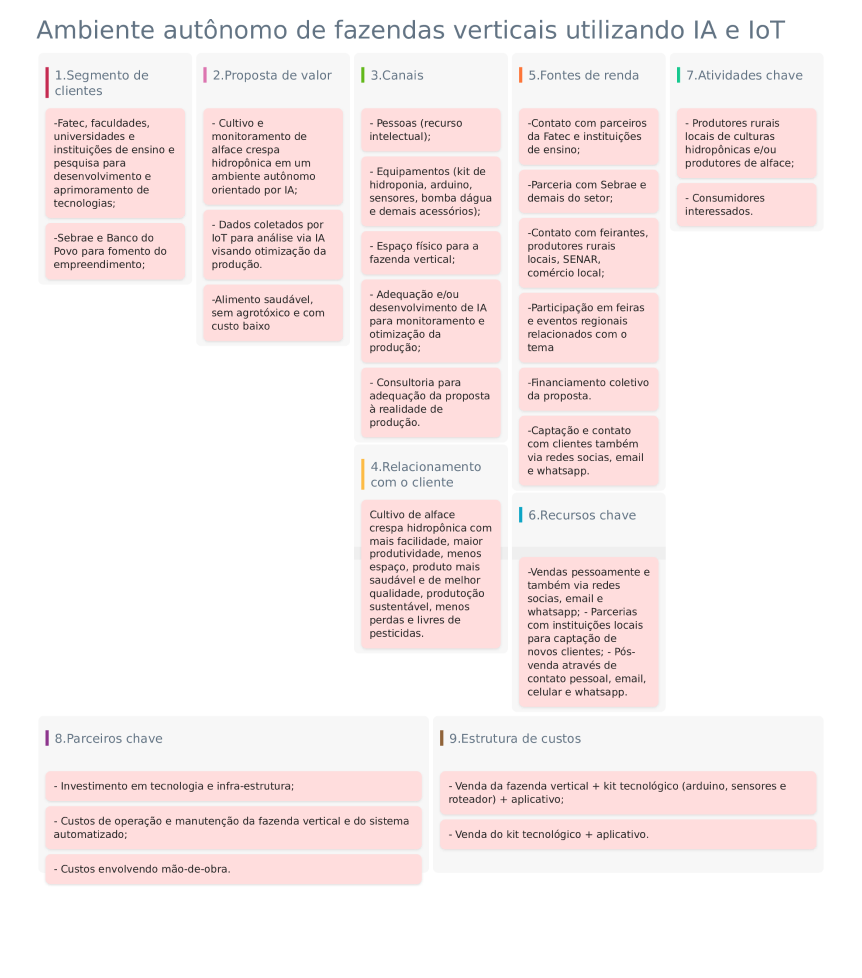
\includegraphics[scale=0.9]{PI - CANVAS.png}
\SourceOrNote{Autoria própria (2025)}
\end{figure}

Nosso projeto, focado em fazendas verticais autônomas, busca atingir primeiramente o público de pessoas físicas residentes em São Paulo (capital) e regiões metropolitanas. Dito isto, a proposta foi desenhada de forma a atingir este mercado.

\section*{Diagrama e Especificações de Estrutura de Rede}
\addcontentsline{toc}{section}{Diagrama e Especificações de Estrutura de Rede}
Diagrama e especificações de estrutura de rede são usados para descrever a infraestrutura de rede: o diagrama é uma representação visual que mapeia os componentes e suas conexões, enquanto as especificações são os detalhes técnicos que documentam a configuração da rede.

\begin{figure}[H] % ← TROQUE [!ht] por [H]
\centering
\caption{Diagrama e Especificações de Estrutura de Rede}
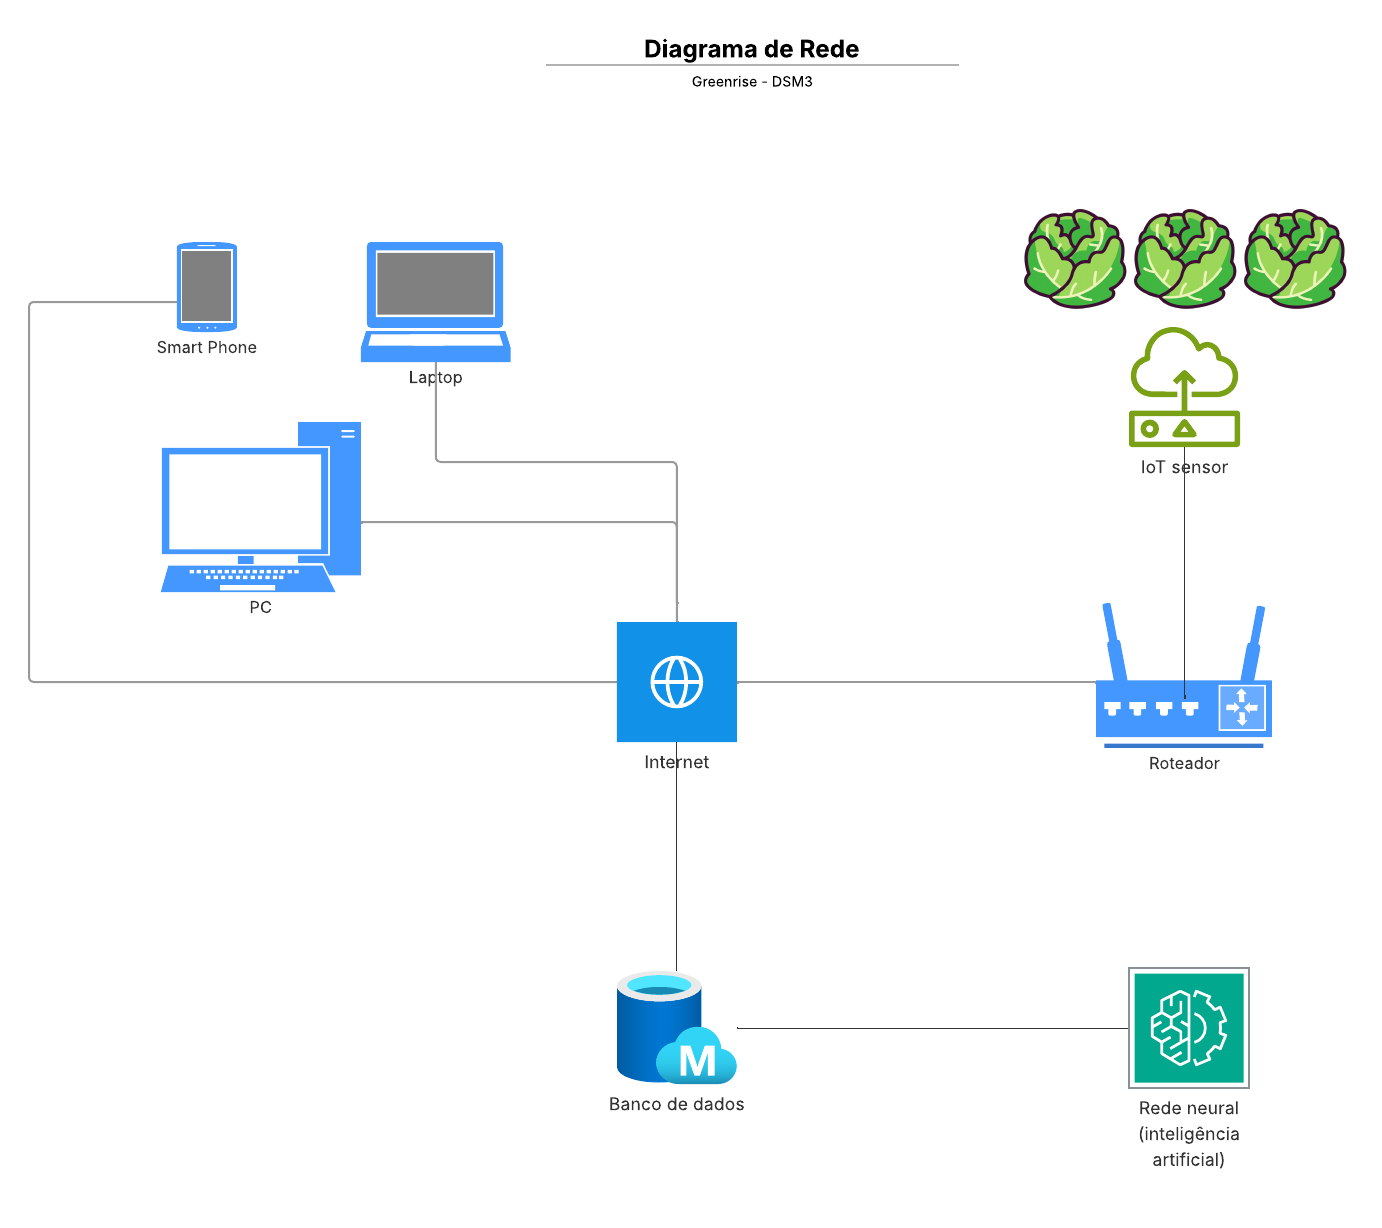
\includegraphics[scale=0.4]{PI - Diagrama de rede.png}
\SourceOrNote{Autoria própria (2025)}
\end{figure}

Considerando o foco em pessoas físicas, nosso projeto considera um ambiente de rede básico envolvendo computadores e celulares como dispositivos de entrada, conexão à internet, banco de dados, uma rede neural, roteador e sensores posicionados na fazenda vertical.

\section*{Analise SWOT}
\addcontentsline{toc}{section}{Analise SWOT}
A Análise SWOT é uma ferramenta de planejamento estratégico que avalia as Forças (Strengths), Fraquezas (Weaknesses), Oportunidades (Opportunities) e Ameaças (Threats) de uma empresa ou projeto.

\begin{figure}[H] % ← TROQUE [!ht] por [H]  
\centering
\caption{Analise SWOT}
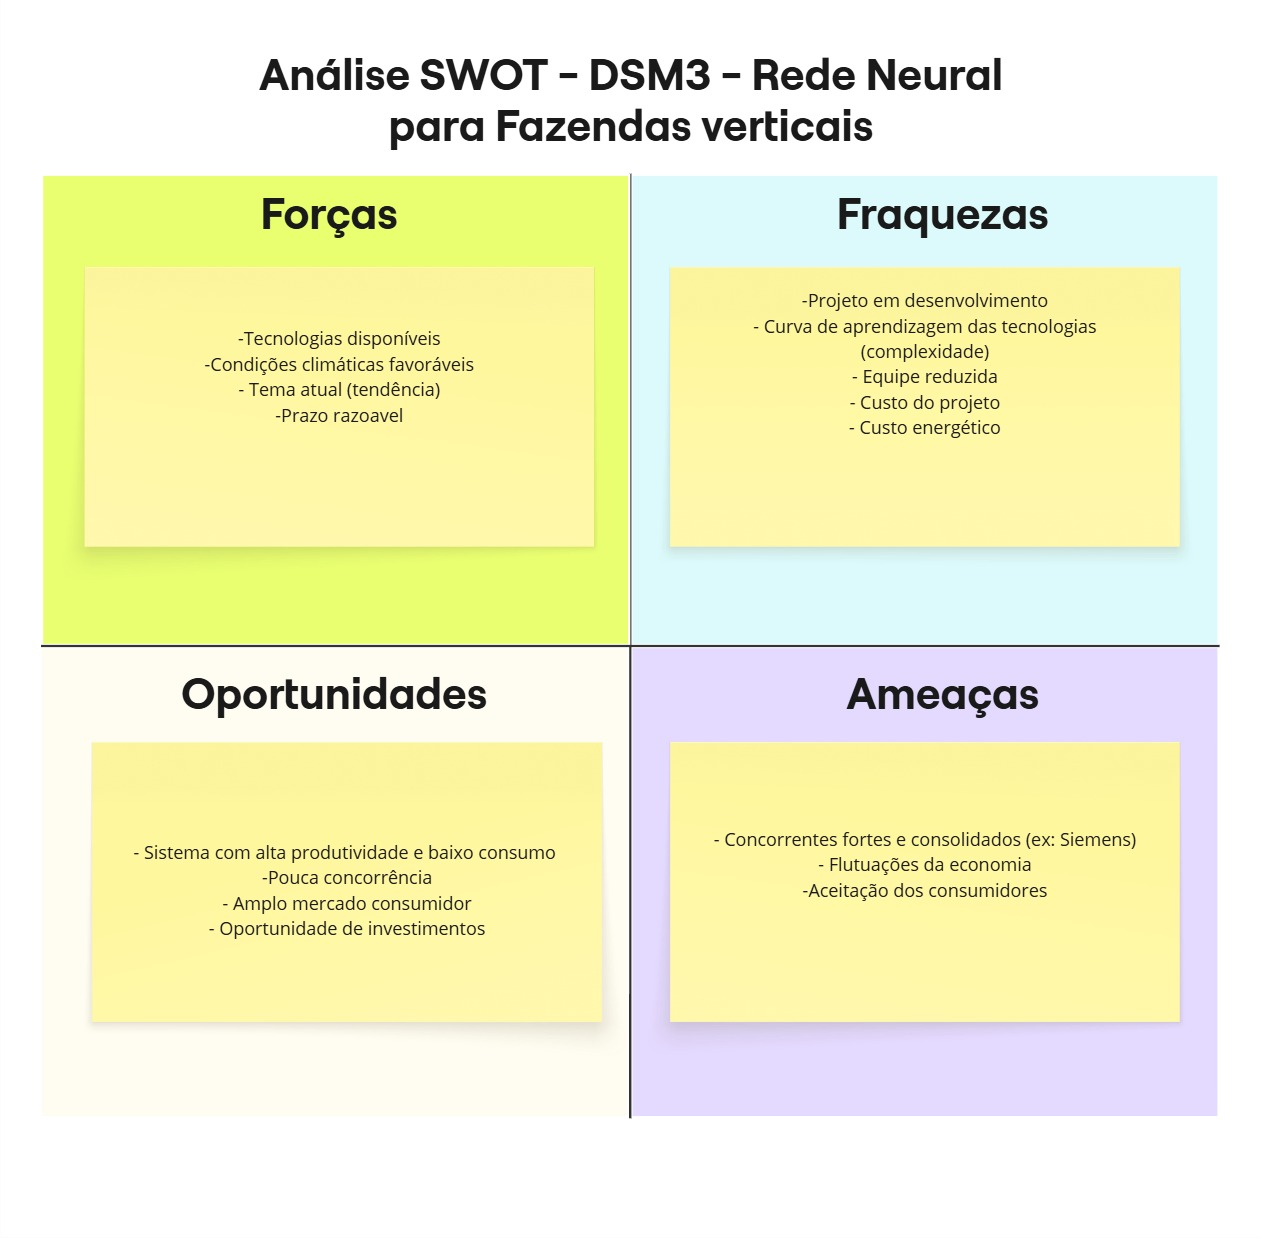
\includegraphics[scale=0.3]{PI - SWOT.jpg}
\SourceOrNote{Autoria própria (2025)}
\end{figure}

As forças e fraquezas se referem ao ambiente interno (controlável), enquanto as oportunidades e ameaças vêm do ambiente externo (não controlável). Essa análise ajuda na tomada de decisões estratégicas e a criar planos de ação mais eficazes. 

\section*{SCRUM}
\addcontentsline{toc}{section}{SCRUM(Kanban)}
Scrum é uma estrutura ágil de gerenciamento de projetos que ajuda equipes a se auto-organizarem para trabalhar em direção a um objetivo comum através de ciclos curtos de trabalho, chamados "sprints".

\begin{figure}[H] % ← TROQUE [!ht] por [H]  
\centering
\caption{SCRUM - Kanban}
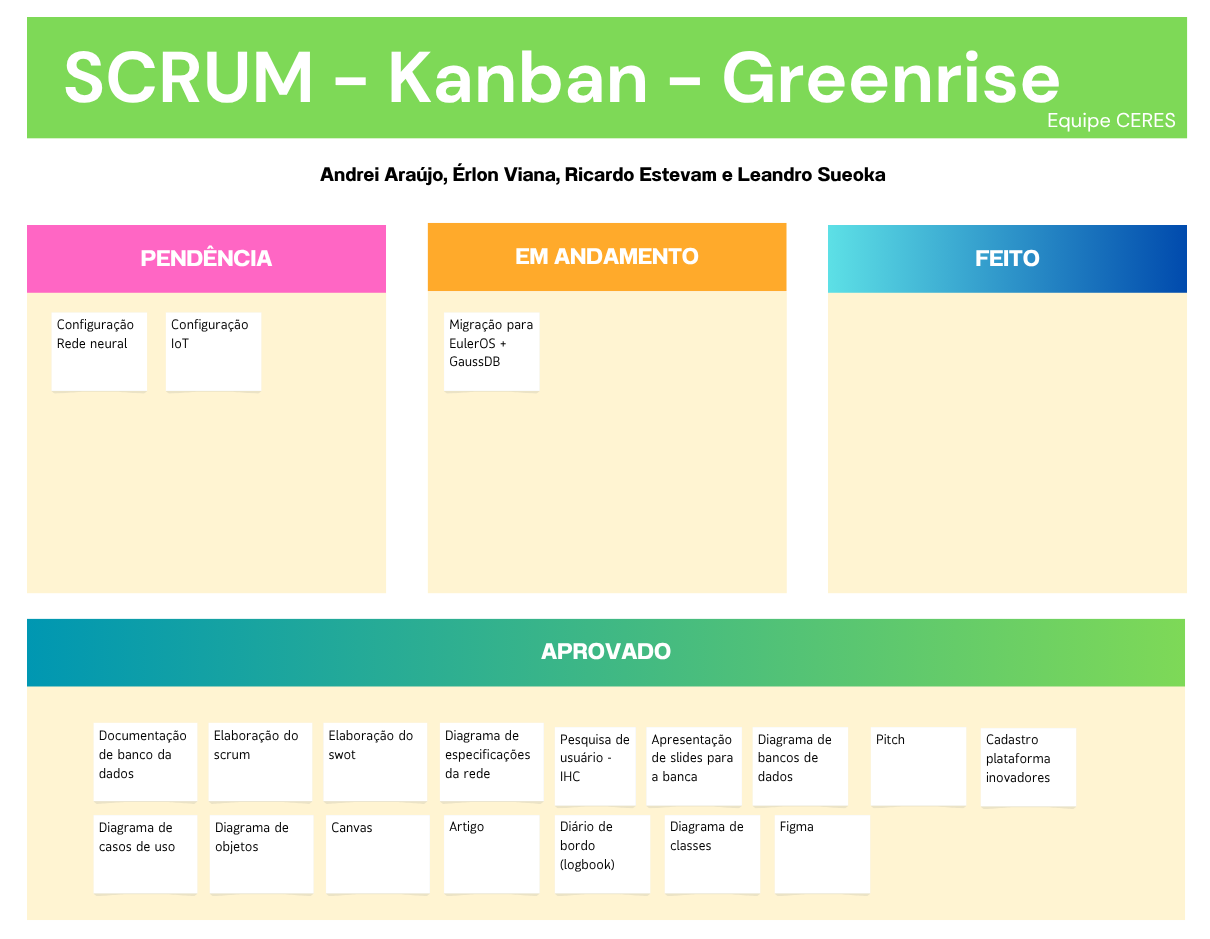
\includegraphics[scale=0.4]{PI - Kanban Greenrise.png}
\SourceOrNote{Autoria própria (2025)}
\end{figure}

Kanban é uma metodologia ágil baseada no conceito visual de gestão de trabalho que usa quadros com colunas e cartões para mostrar o fluxo de tarefas, do início ao fim. Originado na Toyota para a gestão de estoque e produção, o termo japonês significa "sinal visual".

\end{document}